\documentclass[lerntheke,12pt,a5paper,landscape]{arbeitsblatt}

\ladeModule{theme}
\ladeFach[diagramme]{mathematik}

\aboptionen{
	name		= {J. Neugebauer},
	kuerzel 	= {Ngb},
	titel 		= {Lerntheke Terme},
	reihe 		= {Terme},
	fach 		= {Mathematik},
	kurs 		= {5},
	nummer 		= {3},
	lizenz 		= {cc-by-nc-sa-eu-4},
	version 	= {2022-03-07},
	%seitenzahlen= {keine},
}

\usepackage[all]{xy}

\begin{document}


\begin{hilfekarte}{Terme}{terme}
	Einen \emph{sinnvollen} Rechenausdruck aus Zahlen, Rechenzeichen, und Klammern nennen wir einen \textbf{Term}.

	\medskip
	Beispiele:
	\begin{itemize}
		\item $(3 + 15) - 7\cdot 8$
		\item $9283 - 45 : 5$
		\item $1092 - 25\cdot 6 + 95 : 5$
	\end{itemize}

	Wenn in einem Term mehr als zwei Zahlen durch Rechenzeichen verknüpft werden, dann rechnet man nach folgender Vereinbarung:

	\begin{smallenum}
		\item Rechne zuerst den Inhalt von Klammern aus. In den Klammern steht wieder ein Term. Berechne ihn auch nach diesen drei Regeln.
		\item Punkt- vor Strichrechnung.
		\item Kommt nur Punkt- oder nur Strichrechnung vor, rechne von links nach rechts.
	\end{smallenum}
\end{hilfekarte}

\begin{loesungskarte}[Rechenbaum]
	Mit einem Rechenbaum kannst du die Berechnung eines Terms übersichtlich darstellen.

	\[ (53 + 15) - 7\cdot (12 - 4) = \bm{12} \]

\begin{center}
		% \begin{tikzpicture}[num/.style={draw,rectangle},op/.style={draw,circle}]
		% 	\node[num](A) at (-2,0) {$53$};
		% 	\node[num](B) at (0,0) {$15$};
		% 	\node[num](C) at (2,0) {$7$};
		% 	\node[num](D) at (4,0) {$8$};

		% 	\node[op](E) at (-1,-1) {$+$};
		% 	\node[op](F) at (3,-1) {$\cdot$};

		% 	\node[num](G) at (-1,-2) {$71$};
		% 	\node[num](H) at (3,-2) {$56$};

		% 	\node[op](I) at (1,-3) {$-$};
		% 	\node[num](J) at (1,-4) {$15$};

		% 	\draw (A) -- (E) -- (B);
		% 	\draw (C) -- (F) -- (D);
		% 	\draw (E) -- (G);
		% 	\draw (F) -- (H);
		% 	\draw (G) -- (I) -- (H);
		% 	\draw (I) -- (J);
		% \end{tikzpicture}
% ((53+15)-(7*(12-4)))

\centerline{\xymatrix@R=5pt{
  53\ar@{-} `d[1,1] [1,1]&&15\ar@{-} `d[1,-1] [1,-1]&&
    7\ar@{-} '[2,0]+0 `d[3,1] [3,1]&&12\ar@{-} `d[1,1] [1,1]&&4\ar@{-} `d[1,-1] [1,-1]& \\
  &*+[o][F]{+}\ar@{-}[d]&&&&&&*+[o][F]{-}\ar@{-}[d]&& \\
  &*+{68}\ar@{-} '[2,0]+0 `d[3,2] [3,2]&&&&&&*+{8}\ar@{-} `d[1,-2] [1,-2]&
    & \\
  &&&&&*+[o][F]{\txt{$\cdot$}}\ar@{-}[d]&&&& \\
  &&&&&*+{56}\ar@{-} `d[1,-2] [1,-2]&&&& \\
  &&&*+[o][F]{-}\ar@{-}[d]&&&&&& \\
  &&&*+{\bm{12}}&&&&&&
}
}
\end{center}
\end{loesungskarte}

\begin{hilfekarte}{Kommutativgesetz}{kommutativgesetz}\label{hilfe:assoziativgesetz}
Wenn ein term \underline{nur} aus Additionen oder \underline{nur} aus Multiplikationen besteht, dann kannst du die Summanden oder Faktoren beliebig vertauschen.

\begin{multicols}{3}
	$3 + 4 = 4 + 3$

	$8\cdot 7\cdot 9 = 9\cdot 8\cdot 7$

	$5 + 7 + 9 + 12 = 7 + 12 + 5 + 9$
\end{multicols}

\vspace{1cm}
\begin{center}
\begin{tikzpicture}
	\tikzBall(0,0){.2}[red] \tikzBall(.5,0){.2}[red]
	\tikzBall(1.2,0){.2}[blue] \tikzBall(1.7,0){.2}[blue] \tikzBall(2.2,0){.2}[blue] \tikzBall(2.7,0){.2}[blue]

	\tikzBall(3.7,0){.2}[blue] \tikzBall(4.2,0){.2}[blue] \tikzBall(4.7,0){.2}[blue] \tikzBall(5.2,0){.2}[blue]
	\tikzBall(5.9,0){.2}[red] \tikzBall(6.4,0){.2}[red]

	\node at (.25, -1) {$2$};
	\node at (.85, -1) {$+$};
	\node at (1.95, -1) {$4$};
	\node at (3.2,-1) {$=$};
	\node at (4.45, -1) {$4$};
	\node at (5.55, -1) {$+$};
	\node at (6.15, -1) {$2$};
\end{tikzpicture}
\end{center}

\vspace{1cm}
\begin{center}
	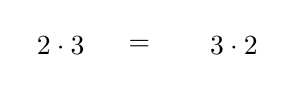
\begin{tikzpicture}
		\tikzBall(0,.5){.2} \tikzBall(.5,.5){.2} \tikzBall(1.0,.5){.2}
		\tikzBall(0,0){.2} \tikzBall(.5,0){.2} \tikzBall(1.0,0){.2}

		\tikzBall(2,.5){.2} \tikzBall(2.7,.5){.2} \tikzBall(3.4,.5){.2}
		\tikzBall(2,0){.2} \tikzBall(2.7,0){.2} \tikzBall(3.4,0){.2}

		\node at (.5, -1) {$2\cdot 3$};
		\node at (1.5,-1) {$=$};
		\node at (2.7, -1) {$3\cdot 2$};
	\end{tikzpicture}
	\end{center}
\end{hilfekarte}

\begin{loesungskarte}[Assoziativgesetz]
\end{loesungskarte}

\begin{hilfekarte}{Distributivgesetz}{distributivgesetz}

\end{hilfekarte}

\begin{loesungskarte}%[Titel H2]
\end{loesungskarte}

\begin{hilfekarte}{Potenzen}{potenzen}

\end{hilfekarte}

\begin{loesungskarte}%[Titel H3]
\end{loesungskarte}




\begin{karte1}{Terme ausrechnen I}
	\hilfeMarke{terme}
	Erstelle einen Rechenbaum und berechne die Lösung der Terme.

	\begin{tasks}(3)
		\task $12 - (7 - 2)$
		\task $120 : (4\cdot  15)$
		\task $4\cdot (25 : (13:3))$
		\task $(25-13) : (11-7)$
		\task $22 : (33 : (5-2))$
		\task $50 : [30 - (25-5)]$
	\end{tasks}
\end{karte1}

\begin{loesungskarte}{Lösung 1}

\end{loesungskarte}

\begin{karte2}{Terme ausrechnen II}
	\hilfeMarke{terme}
	Berechne die Lösung der Terme.
\end{karte2}

\begin{loesungskarte}{Lösung 2}

\end{loesungskarte}

\begin{karte1}{Rechenvorteile nutzen}

\end{karte1}

\begin{loesungskarte}{Lösung 3}

\end{loesungskarte}

\begin{karte1}{Ausklammern}

\end{karte1}

\begin{loesungskarte}{Lösung 4}

\end{loesungskarte}

\begin{karte1}{Ausmultiplizieren}

\end{karte1}

\begin{loesungskarte}{Lösung 5}

\end{loesungskarte}

\begin{karte2}{Distributivgesetz}

\end{karte2}

\begin{loesungskarte}{Lösung 6}

\end{loesungskarte}

\begin{karte2}{Geschickt rechnen}

\end{karte2}

\begin{loesungskarte}{Lösung}

\end{loesungskarte}

\begin{karte1}{Potenzieren}

\end{karte1}

\begin{loesungskarte}{Lösung}

\end{loesungskarte}


\end{document}
